% !TeX spellcheck = es_ES
\documentclass[12pt, titlepage]{article}
\usepackage[nottoc,notlot,notlof,numbib]{tocbibind}
\usepackage[letterpaper, margin=2.5cm]{geometry}
\usepackage[utf8]{inputenc}
\usepackage[spanish]{babel}
\usepackage{listings}
% imagenes
\usepackage{graphicx} 
\usepackage{float}
% fin imagenes
\usepackage{url}
\usepackage{color}

\definecolor{dkgreen}{rgb}{0,0.6,0}
\definecolor{gray}{rgb}{0.5,0.5,0.5}
\definecolor{mauve}{RGB}{253,151,31}
\definecolor{deepred}{RGB}{249,38,114}

\lstset{frame=tb,
	language=MATLAB,
	aboveskip=3mm,
	belowskip=3mm,
	showstringspaces=false,
	columns=flexible,
	numbers=left,
	stepnumber=1,
	basicstyle={\small\ttfamily},
	numberstyle=\tiny\color{gray},
	keywordstyle=\color{blue},
	commentstyle=\color{dkgreen},
	stringstyle=\color{mauve},
	breaklines=true,
	breakatwhitespace=true,
	tabsize=2,
	morekeywords={self, append},
	emph={},
	emphstyle=\color{deepred}
}

\title{Reporte}
\author{Barrera Pérez Carlos Tonatihu \\ Profesor: Moreno Armendariz Marco Antonio \\ Redes Neuronales \\ Grupo: 3CM2 }
\begin{document}
    \maketitle
    \tableofcontents
    \newpage
    \section{Introducción}
        Este reporte es sobre tres distintas arquitecturas de redes neuronales, las cuales son: Hamming Perceptron Simple y ADALINE. Se incluye una breve explicación sobre estas arquitecturas el como funcionan y sus diferentes representaciones para que sea fácil de entender.
        \\\\
        Además, se programaron estas tres arquitecturas, sujetas a algunas restricciones para que fuera más sencilla su elaboración, el desarrollo de estos programas fue realizado en \emph{MATLAB} ya que nos proporciona un manejo sencillo de matrices, lo cual es el principal elemento con el que trabajan estas redes neuronales. 
        \\\\
        Para verificar el correcto funcionamiento de los programas se realizaron pruebas con entradas de diferentes tamaños y valores, de igual forma se muestra en pantalla el resultado y una representación gráfica. Para complementar los resultados obtenidos se incluye un análisis de estos.
        \\\\
        Finalmente, tenemos una sección de conclusiones sobre la parte más importante de este reporte.
    \section{Marco teórico}
        \subsection{Hamming}
        Hamming es una mamada \cite{libro1}
        \subsection{Perceptron}
        \subsection{ADALINE}
    \section{Resultados experimentales}
        \subsection{Hamming}
            \begin{figure}[H]
                \begin{center}
                    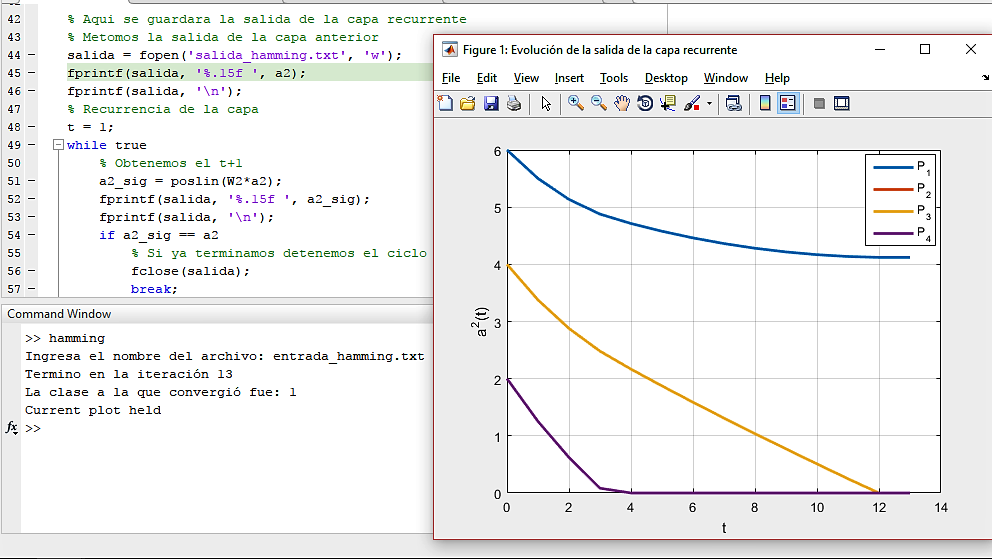
\includegraphics[width=16cm]{img/hamming1.png}
                    \caption{Prueba 1 de la red Hamming.}
                    \label{fig:hamming1}
                \end{center}
            \end{figure}
        
            \begin{figure}[H]
                \begin{center}
                    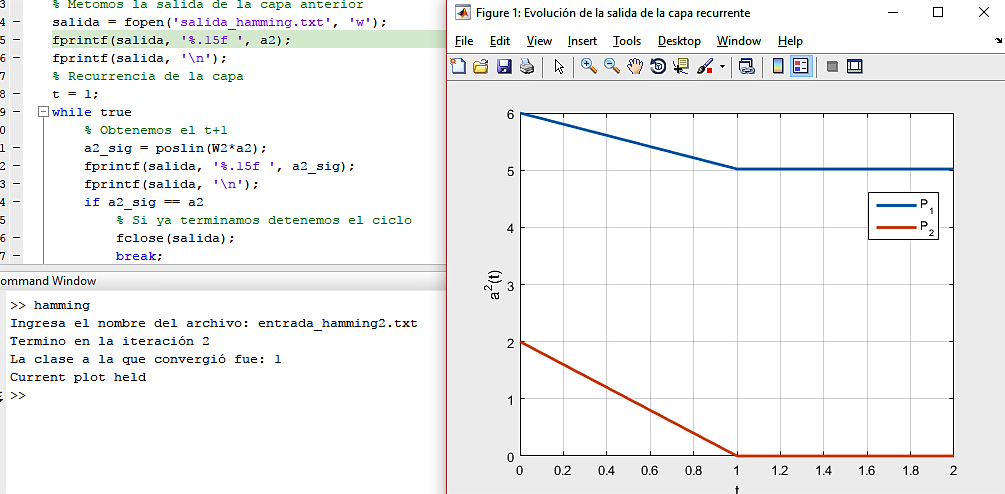
\includegraphics[width=16cm]{img/hamming2.png}
                    \caption{Prueba 2 de la red Hamming.}
                    \label{fig:hamming2}
                \end{center}
            \end{figure}
        
            \begin{figure}[H]
                \begin{center}
                    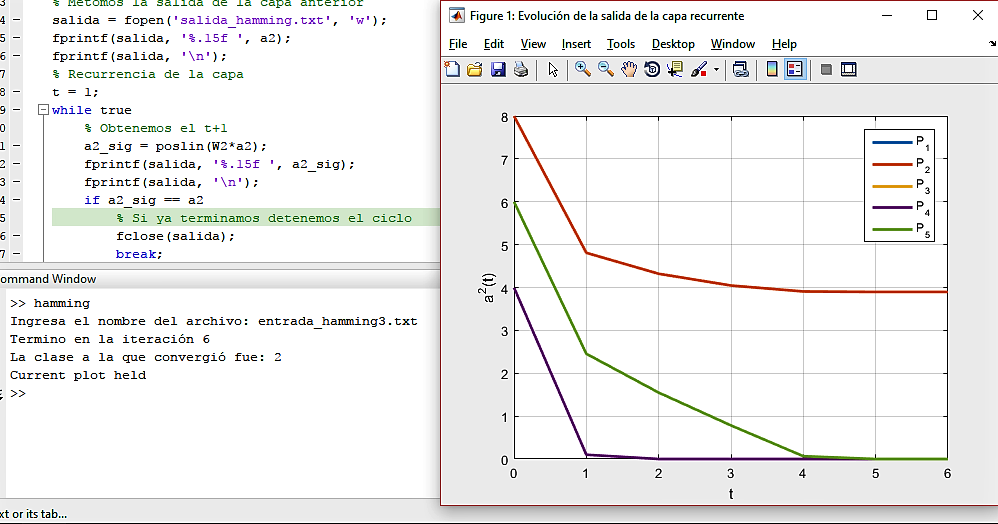
\includegraphics[width=16cm]{img/hamming3.png}
                    \caption{Prueba 3 de la red Hamming.}
                    \label{fig:hamming3}
                \end{center}
            \end{figure}
        \subsection{Perceptron}
            \subsubsection{Método Gráfico}
            \subsubsection{Aprendizaje}
        \subsection{ADALINE}
            \subsubsection{Con bias}
            \subsubsection{Sin bias}
    \section{Discusión de resultados}
        \subsection{Hamming}
        \subsection{Perceptron}
        \subsection{ADALINE}
    \section{Conclusiones}
    \bibliographystyle{apalike}
    \bibliography{bibliografia}
    \section{Anexo}
        En esta sección se encuentra el código de los tres programas desarrollados en MATLAB.
        \subsection{Hamming}
        \begin{lstlisting}
% Cada elemento del vector de entrada tiene solo dos posibles valores
opcion = input('Ingresa el nombre del archivo: ', 's');
archivo = dlmread(opcion);
tam = size(archivo);
% Tam de nuestros vectores prototipo
R = tam(2);

% Numero de neuronas, corresponde a cada vector prototipo
S = tam(1) - 1;

% Vector a clasificar
p = archivo(S+1, :)';

% Las filas de W1 son los vectores prototipos
% Inicializacion de W1
W1 = archivo(1:S, :);

% Cada elemento del bias es el tam del vector prototipo
% Inicializacion del bias
b1 = ones(S, 1) * R;

% Propagamos hacia adelante
a1 = purelin((W1*p)+b1);
% Fin de la capa feedforward

%Inicio de la capa recurrente
a2 = a1;
% Obtencion del valor epsilon 0 < epsilon < 1/(S-1)
epsilon = round(rand(1)*1/(S-1), 4); 
% Inicializacion y llenado de la W2 de la capa recurrente
W2 = ones(S, S);
for i = 1:S
    for j = 1:S
        if i==j
            W2(i, j) = 1;
        else
            W2(i, j) = -epsilon; 
        end;
    end;
end;

% Aqui se guardara la salida de la capa recurrente
% Metomos la salida de la capa anterior
salida = fopen('salida_hamming.txt', 'w');
fprintf(salida, '%.15f ', a2);
fprintf(salida, '\n');
% Recurrencia de la capa
t = 1;
while true
    % Obtenemos el t+1
    a2_sig = poslin(W2*a2);
    fprintf(salida, '%.15f ', a2_sig);
    fprintf(salida, '\n');
    if a2_sig == a2
        % Si ya terminamos detenemos el ciclo
        fclose(salida);
        break;
    else
        % Siguiente iteracion
        a2 = a2_sig;
    end;
    t = t + 1;
end;

% Fin de la capa recurrente
fprintf('Termino en la iteracion %d\n', t);
v = 1;
for ite = a2'
    if ite ~= 0
        break;
    else
        v = v+1;
    end;
end
fprintf('La clase a la que convergio fue: %d\n', v);
% Imprimir datos y graficar la salida de a2
a2_recurrente = dlmread('salida_hamming.txt');
figure('Name', 'Evolucion de la salida de la capa recurrente');
plot(0:t, a2_recurrente, 'LineWidth', 2);
hold;
grid;
xlabel('t');
ylabel('a^2(t)');
etiquetas = cell(1, S);
for i = 1:S
    etiquetas{i} = ['P_' num2str(i)];
end;
legend(etiquetas);
        \end{lstlisting}
        \subsection{Perceptron}
        \subsection{ADALINE}
\end{document}